\setlength{\columnsep}{20pt}
\begin{flushleft}
	There are 3 types of OS:
	\begin{enumerate}
		\item 
		\begin{multicols}{2}
			\textbf{Server OS} - Designed for server computers that runs 24X7.
			\newline
			Eg:
			\begin{itemize}
				\item Linux server
				\item Windows server
				\item Mac OS X server
			\end{itemize}
			\vfill \null
			\columnbreak
			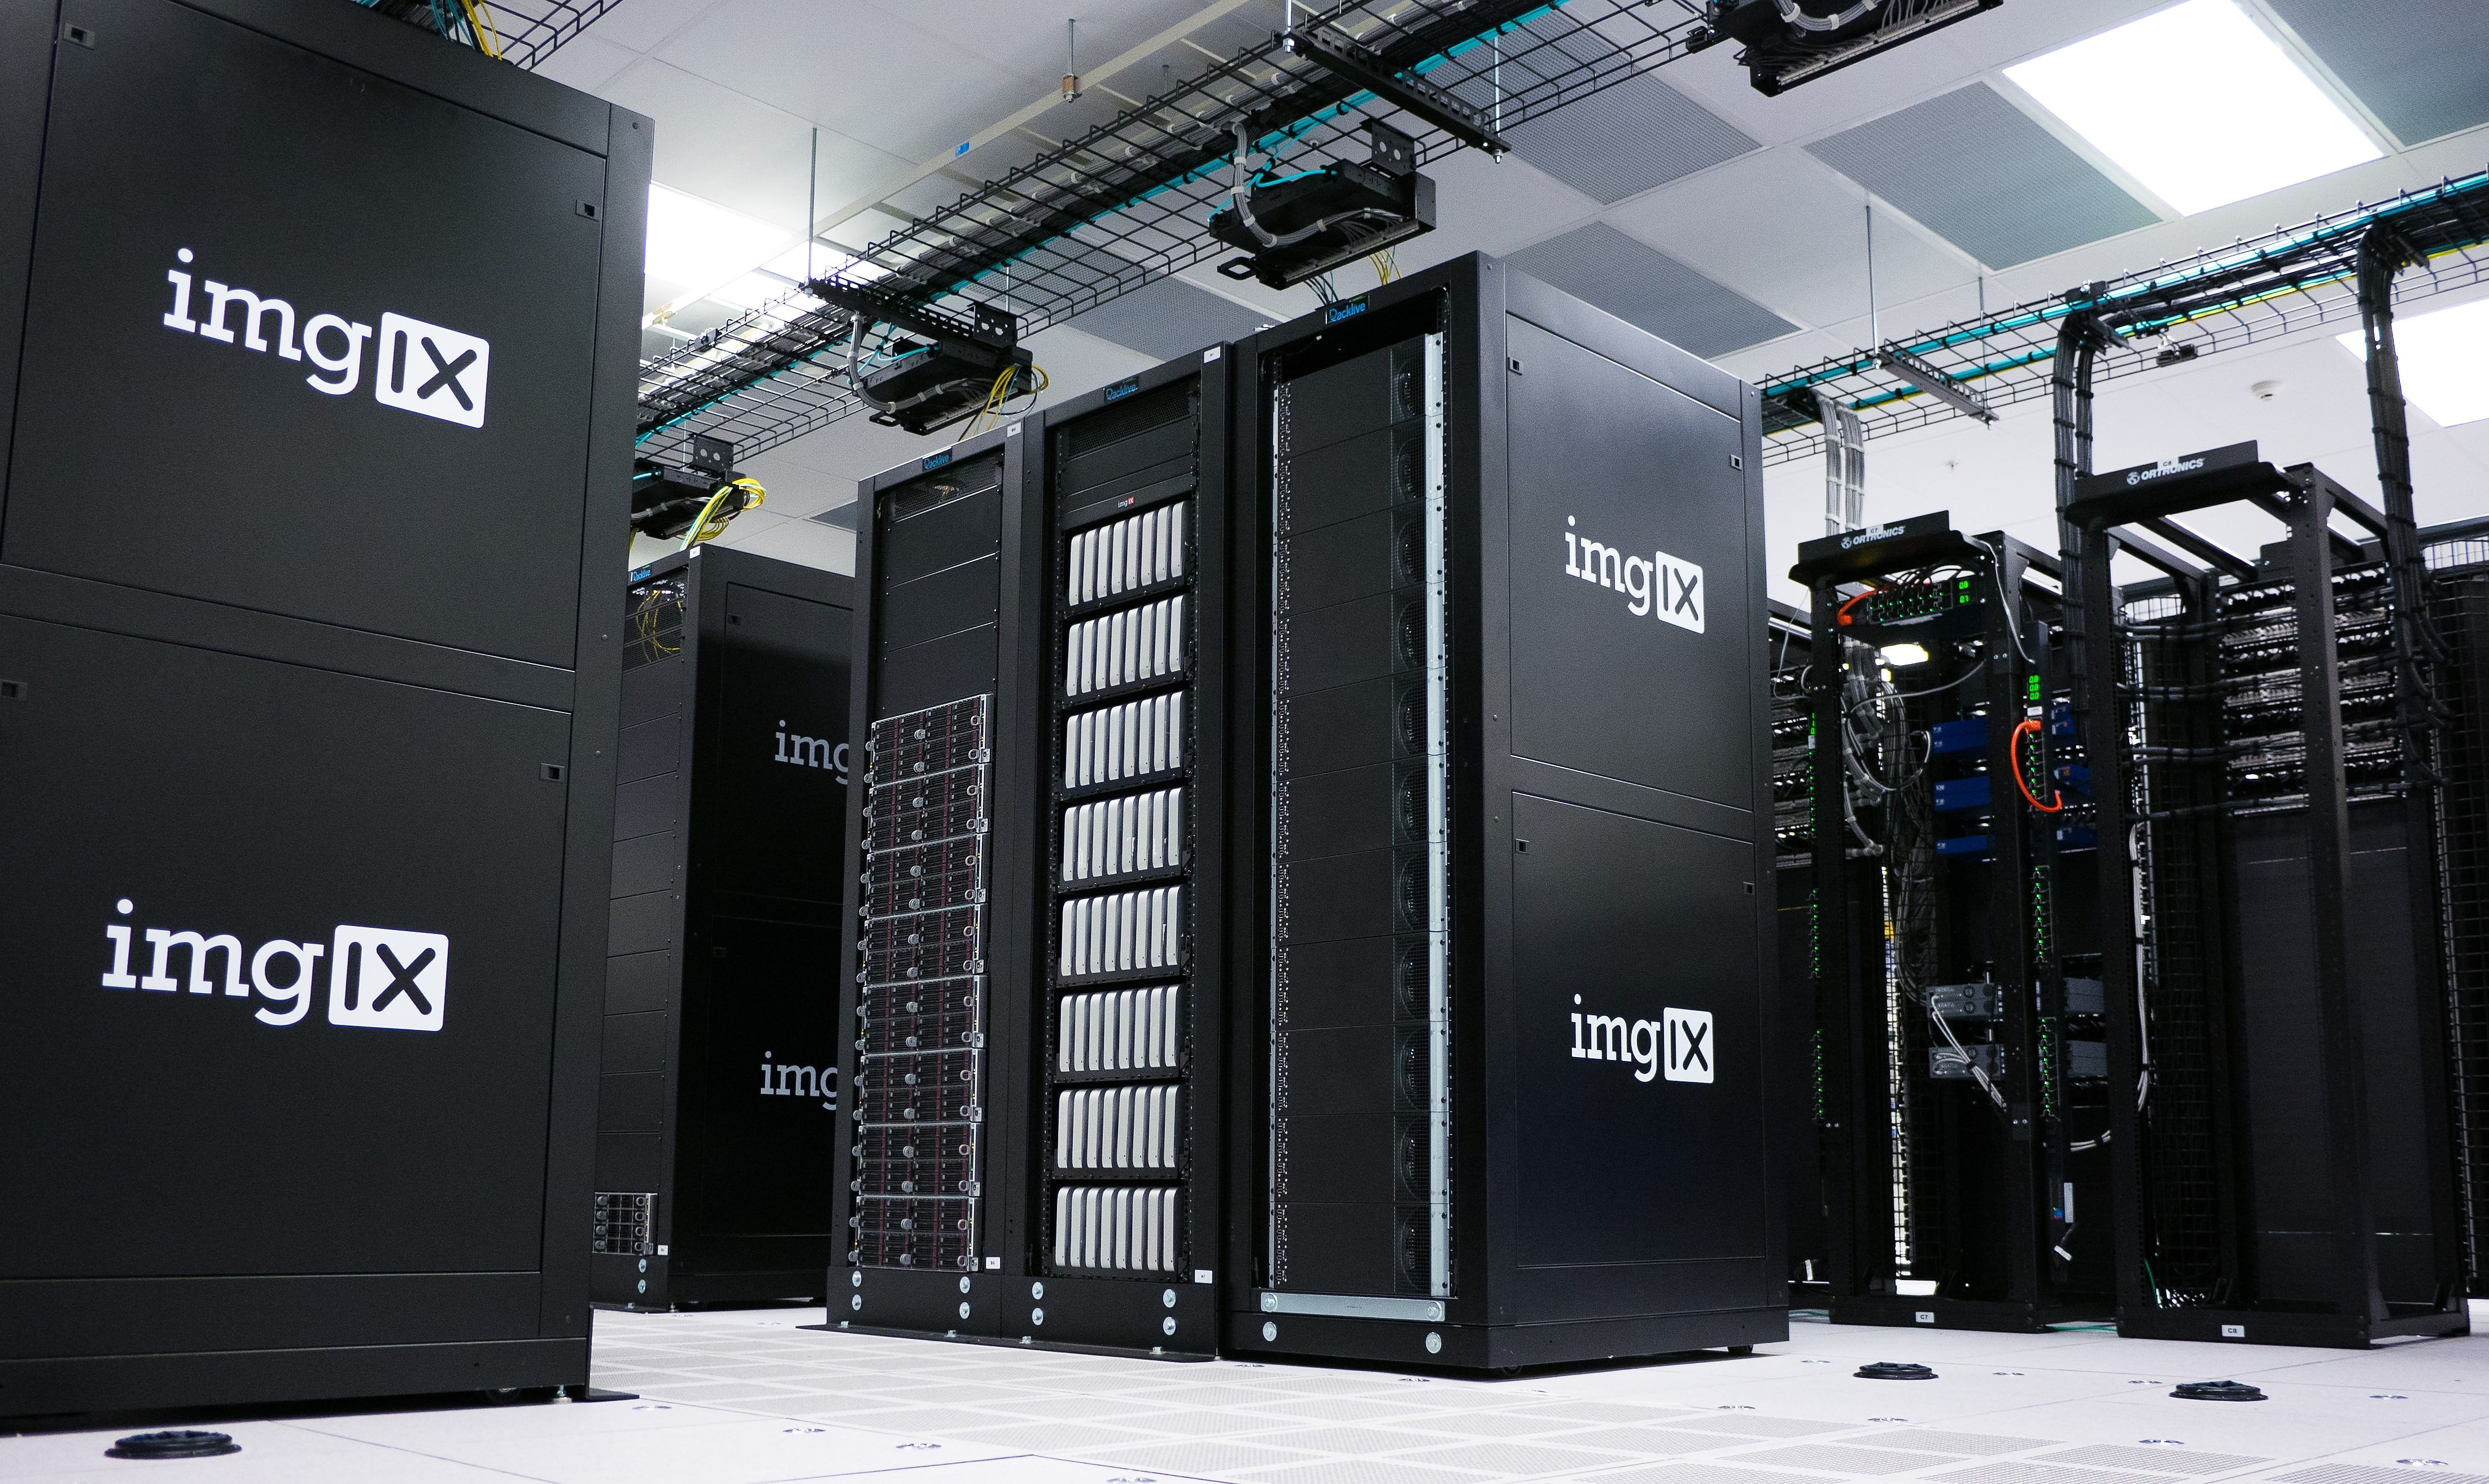
\includegraphics[scale=.03]{content/chapter1/images/server.jpg}
		\end{multicols}
		\vspace{-25pt}

\bigskip
		
		\item 
		\begin{multicols}{2}
			\textbf{Desktop OS} - Designed for personal computer.
			\newline
			Eg:
			\begin{itemize}
				\item Windows
				\item Mac OS
			\end{itemize}
			\vfill \null			
			\columnbreak
			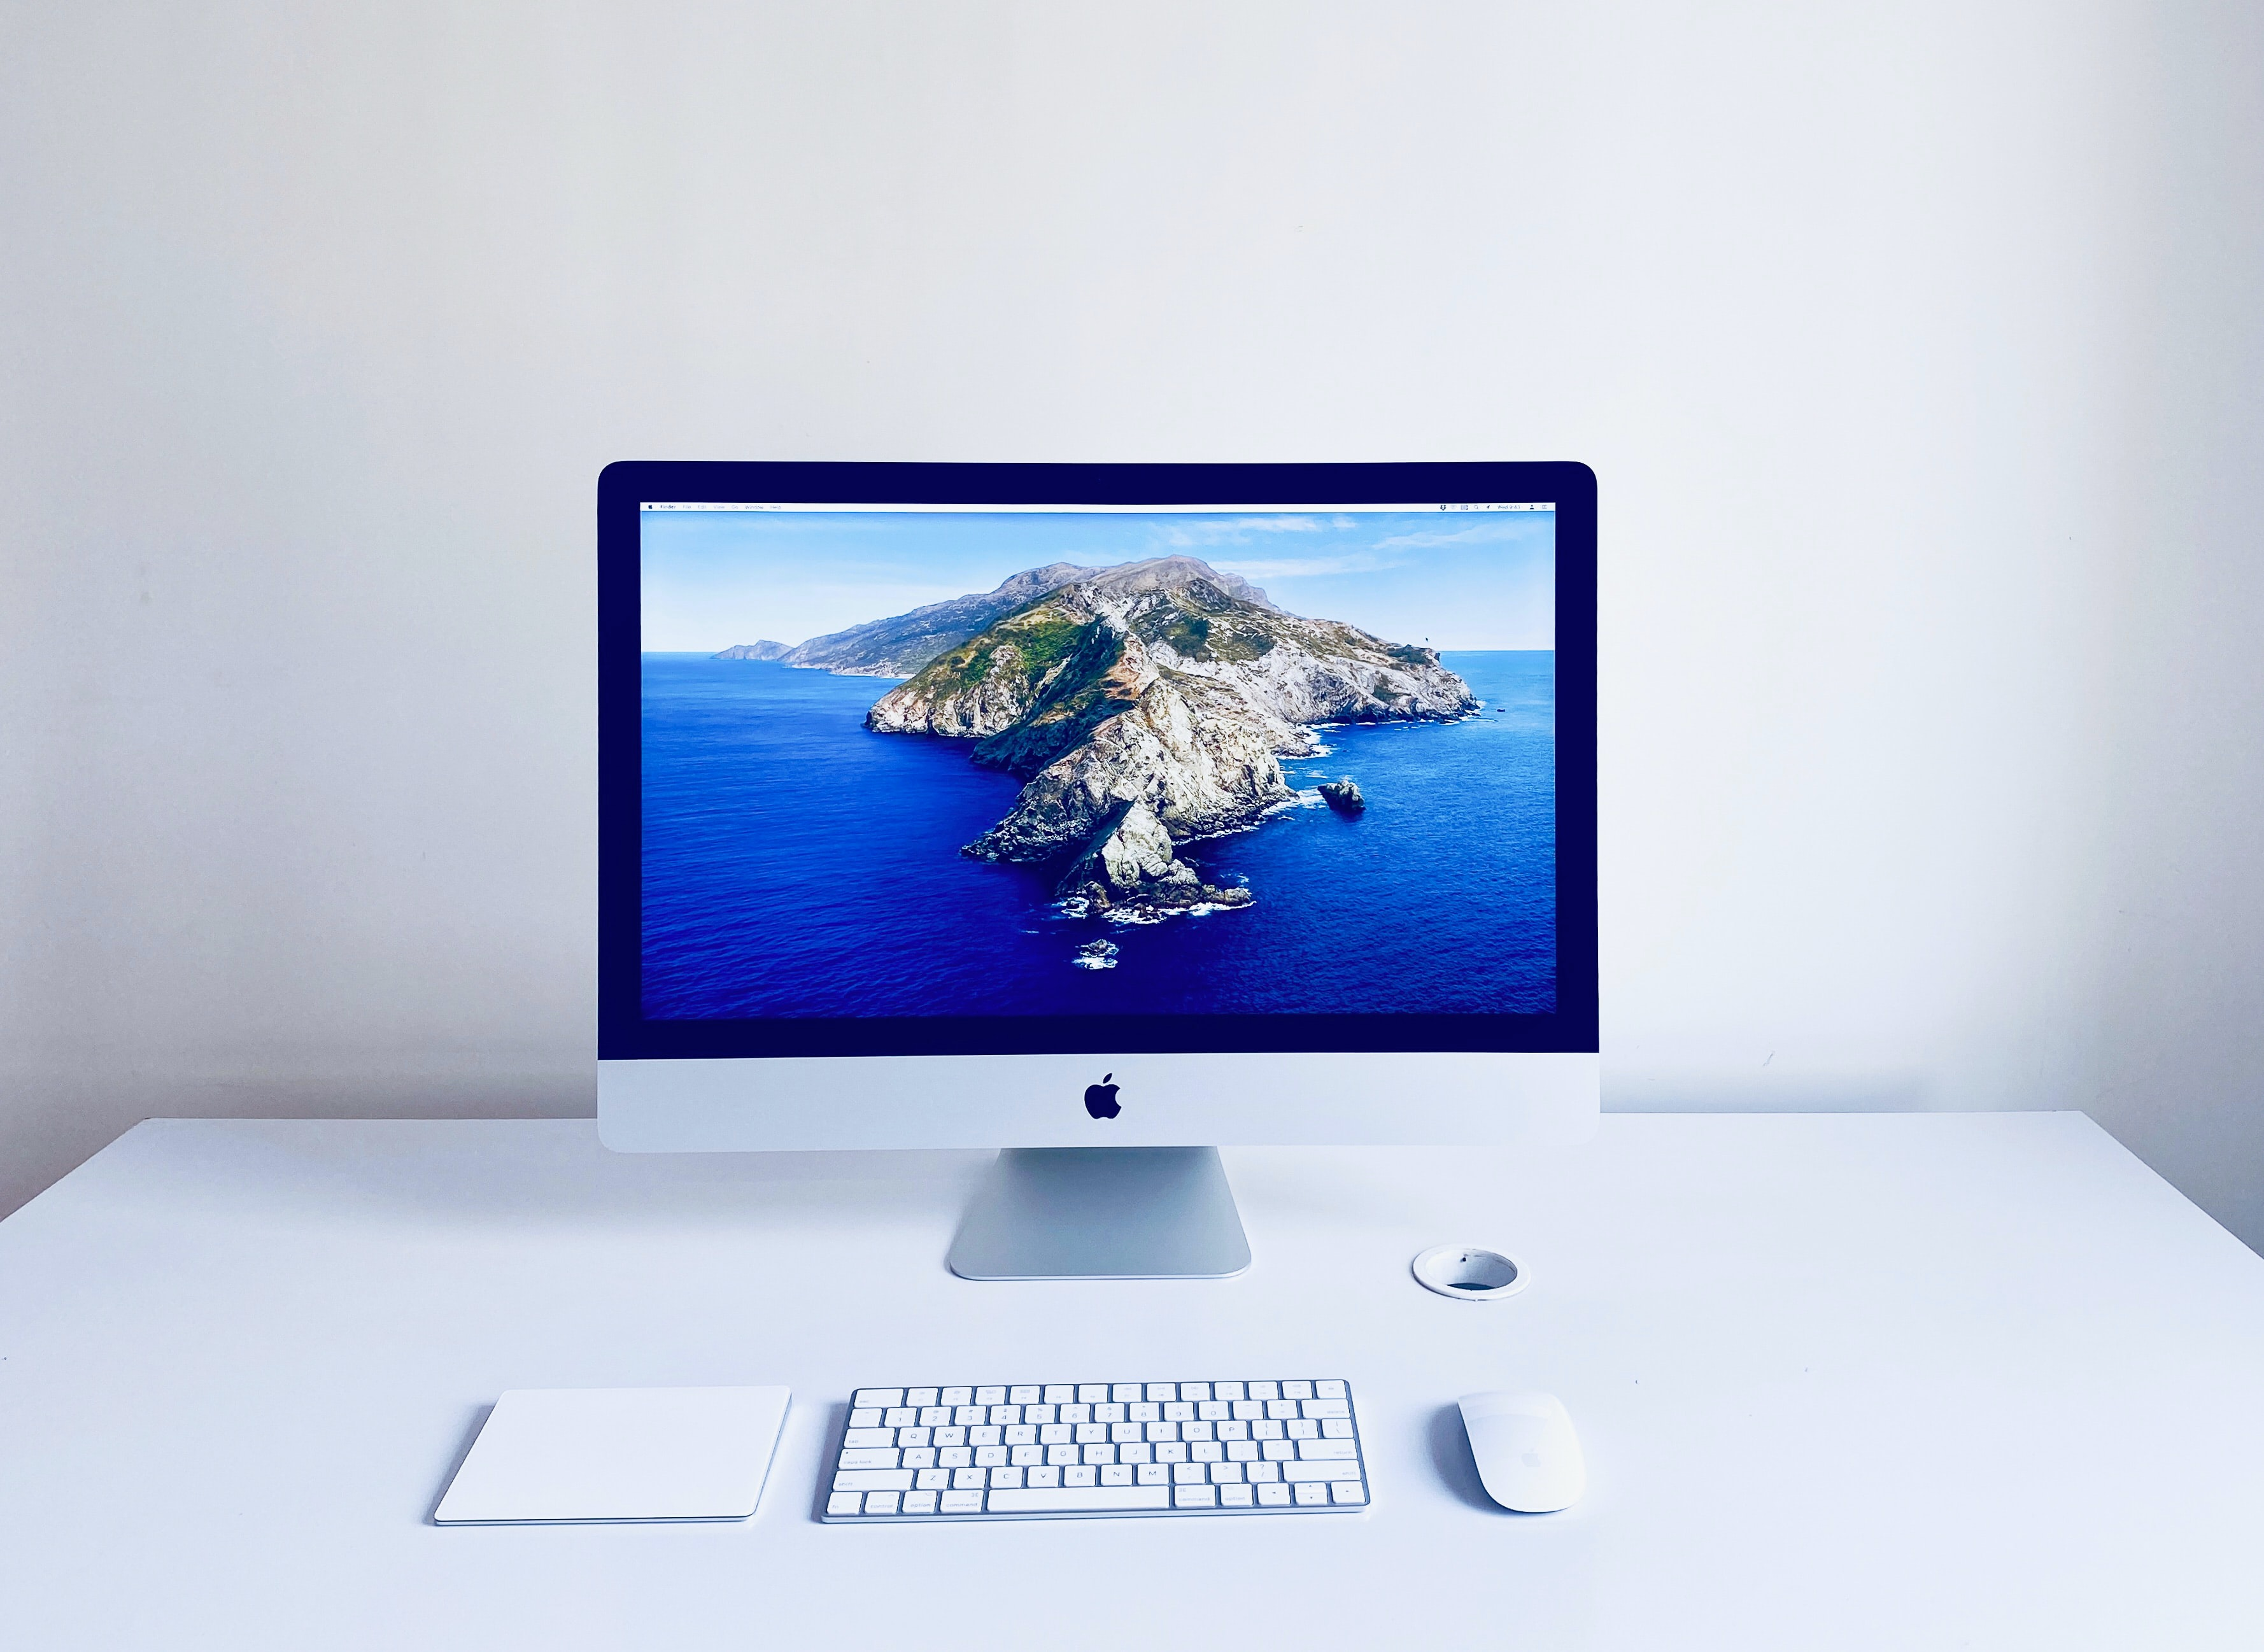
\includegraphics[scale=.03]{content/chapter1/images/desktop.jpg}
		\end{multicols}
		\vspace{-25pt}
		
\bigskip
		
		\item 
		\begin{multicols}{2}
			\textbf{Mobile OS} - Designed to run on mobile devices.
			\newline
			Eg:
			\begin{itemize}
				\item IPhone OS
				\item Windows mobile
				\item Anroid
			\end{itemize}
			\vfill \null			
			\columnbreak
			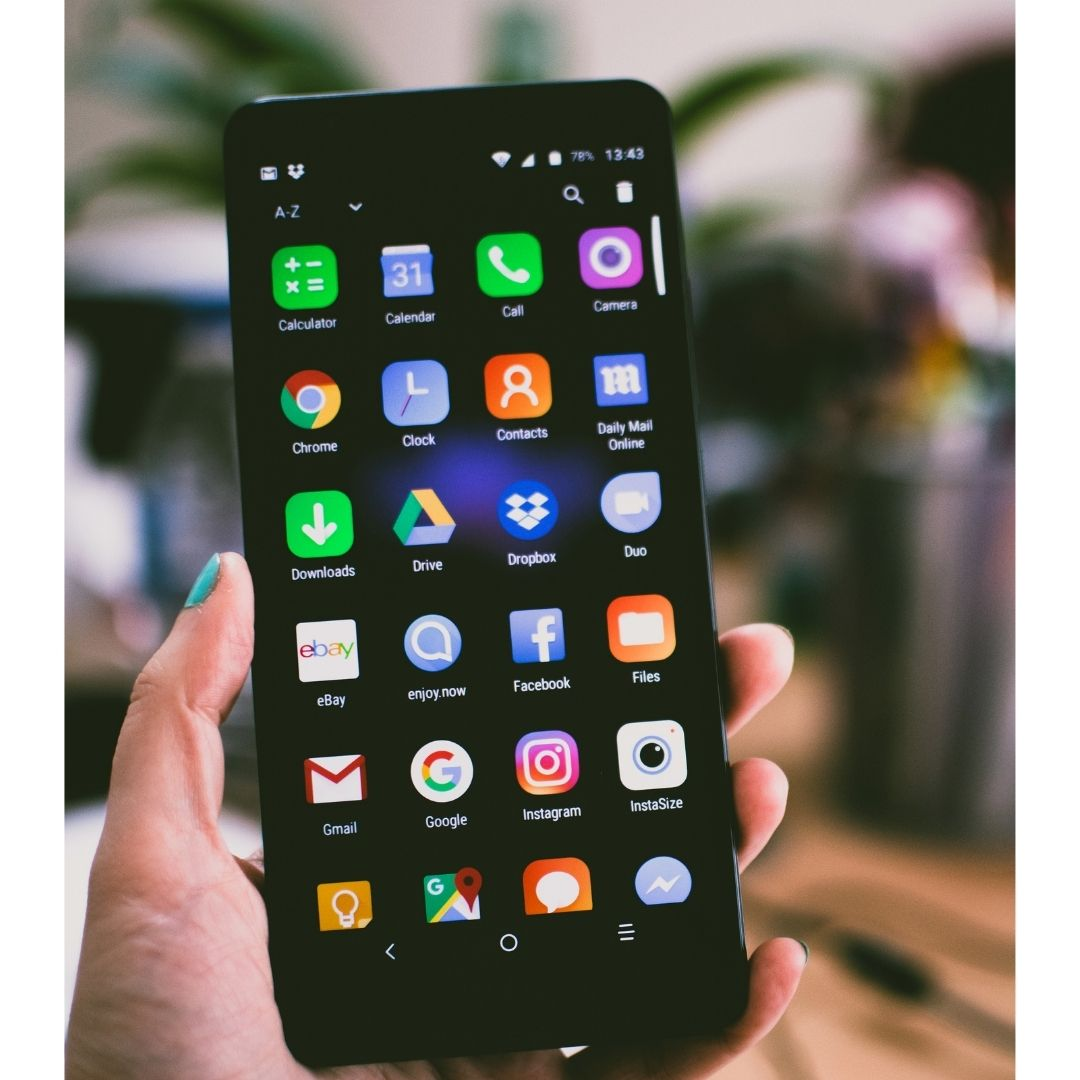
\includegraphics[scale=.12]{content/chapter1/images/mobile.jpg}
		\end{multicols}
		\vspace{-25pt}

		%\bigskip
	\end{enumerate}
\end{flushleft}

\newpage

